\clearpage
\section{Single File Download Times}
\label{sec:evaluation-single-file}

\begin{figure*}[!htb]
    \begin{minipage}[t]{0.8\linewidth}
	\begin{center}
        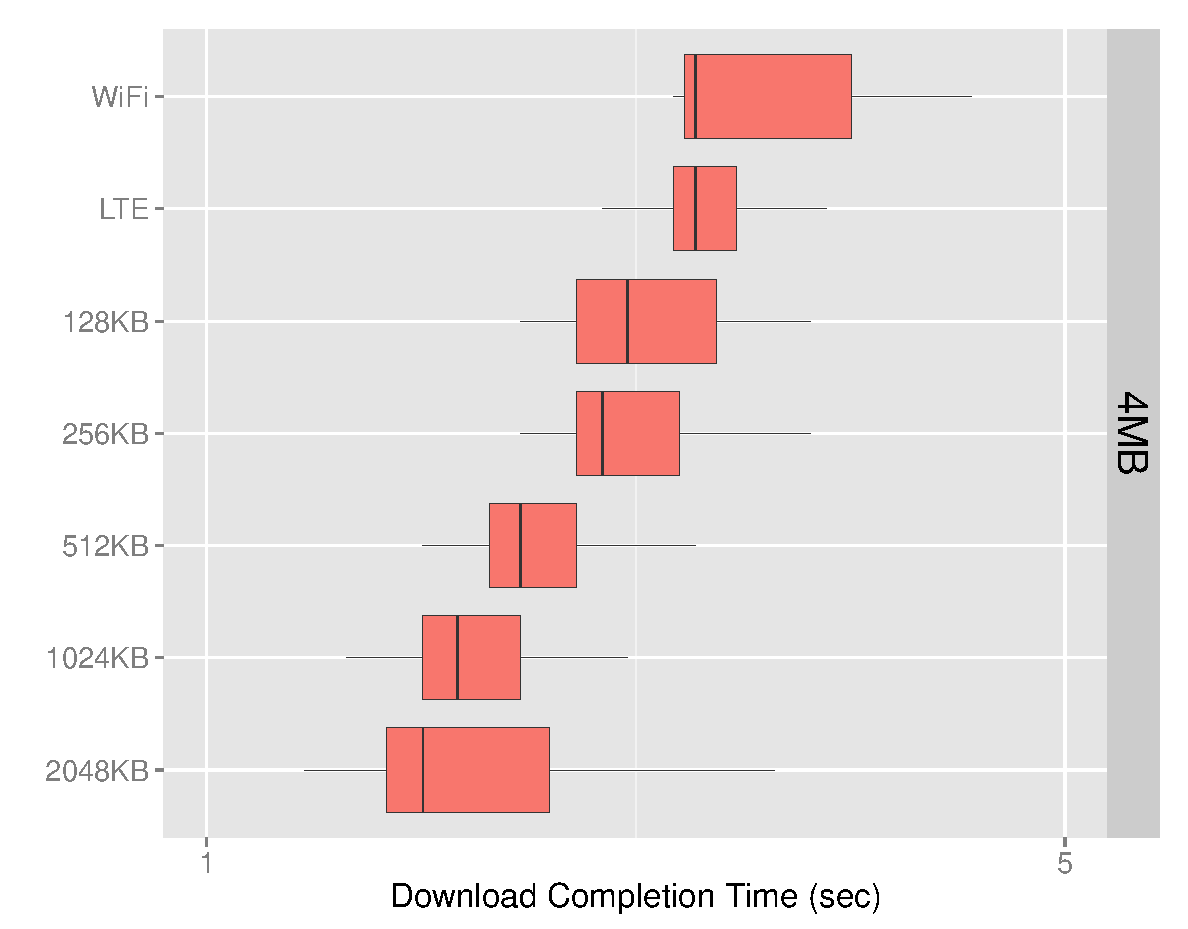
\includegraphics[width=\linewidth]{Figures/baseline-scheduler-us-testbed.pdf}
		\caption{\label{fig:evaluation-baseline-us}\algbase~scheduler results from our US testbed.}
    \end{center}
    \end{minipage}
\vspace*{-0.3cm}
\end{figure*}

We now evaluate the different scheduling approaches for single file downloads, again using the download completion time as the major performance metric. 
We also compare the traffic distributions over the paths. 
In each scenario we measure over $30$ rounds, with each round having a randomized configuration sequence in order to account for traffic dependencies and/or correlation. 
We depict the median, $25-75$\perc percentiles (boxes), and the dispersion (lines, $5-95$\perc percentiles). 
As explained in~\xref{sec:evaluation-initial-chunk}, we use an initial chunk size of $32$KB.

\subsection{Baseline Scheduler}
\label{sec:evaluation-baseline}

In~\fref{fig:evaluation-baseline-us} and~\fref{fig:evaluation-baseline-de} we depict the performance of the \algbase~scheduler of \protoold~as described in~\xref{sec:baseline-scheduler}. 
In~\fref{fig:evaluation-baseline-us} we show the results achieved from our collaborators in the US and in~\fref{fig:evaluation-baseline-de} the results in our testbed in Germany. 
Here, we only illustrate the results of a $4$MB file download, since we only want to emphasize that the optimal fixed chunk size differs from testbed to testbed. 
Deeper studies on the \protoold~\algbase~scheduler for different file sizes have already been performed in the previous research~\cite{KIM13-MHTTP}.

\begin{figure*}[!htb]
    \begin{minipage}[t]{0.8\linewidth}
    \begin{center}
        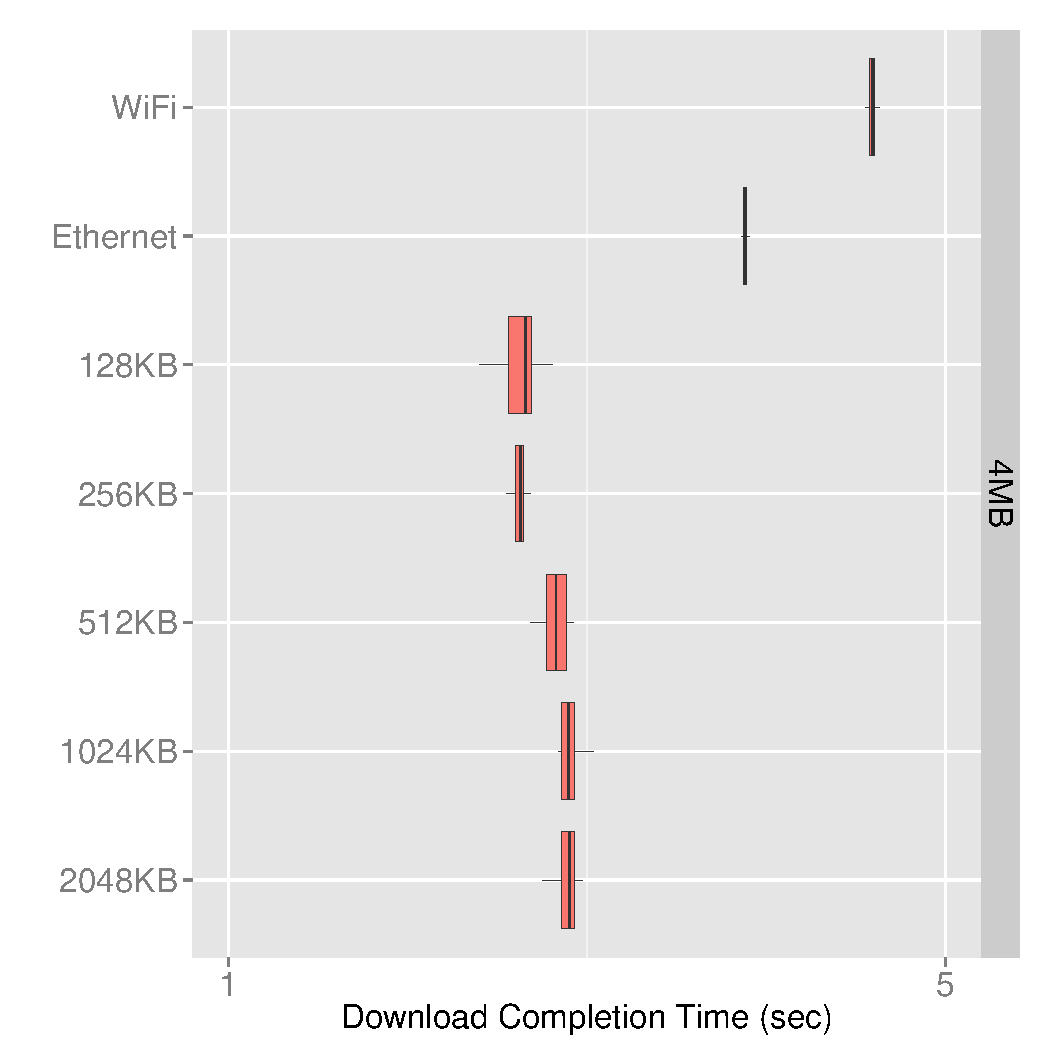
\includegraphics[width=\linewidth]{Figures/baseline-scheduler-de-testbed-4M.pdf}
		\caption{\label{fig:evaluation-baseline-de}\algbase~scheduler results from our German testbed.}
    \end{center}
    \end{minipage}
  \vspace*{-0.3cm}
\end{figure*}

 

In~\fref{fig:evaluation-baseline-us} we can clearly see that the optimal fixed chunk size is $2$MB, whereas in our German testbed in~\fref{fig:evaluation-baseline-de} $128$KB and $256$KB are the optimal fixed chunk sizes. 
When looking at the link qualities in the US testbed, we see that the median throughput is the same. 
An equal distribution of $2$MB chunks on the links performs best, because the request overhead is minimal and both links can more or less handle the same amount of traffic in the same time. 
In contrast to this, we see in our German testbed that both links clearly differ in throughput. 
This proofs that equal traffic distribution might not deliver the optimal result in every case, which is why smaller fixed chunks perform better here, even though they come with a higher request overhead. 

These results perfectly show that the optimal chunk size depends on the link quality and is different from scenario to scenario. 

\pagebreak
\subsection{Implication of $\alpha$ values}
\label{sec:evaluation-alpha}

\begin{figure*}[!htb]
    \begin{minipage}[t]{0.8\linewidth}
	\begin{center}
        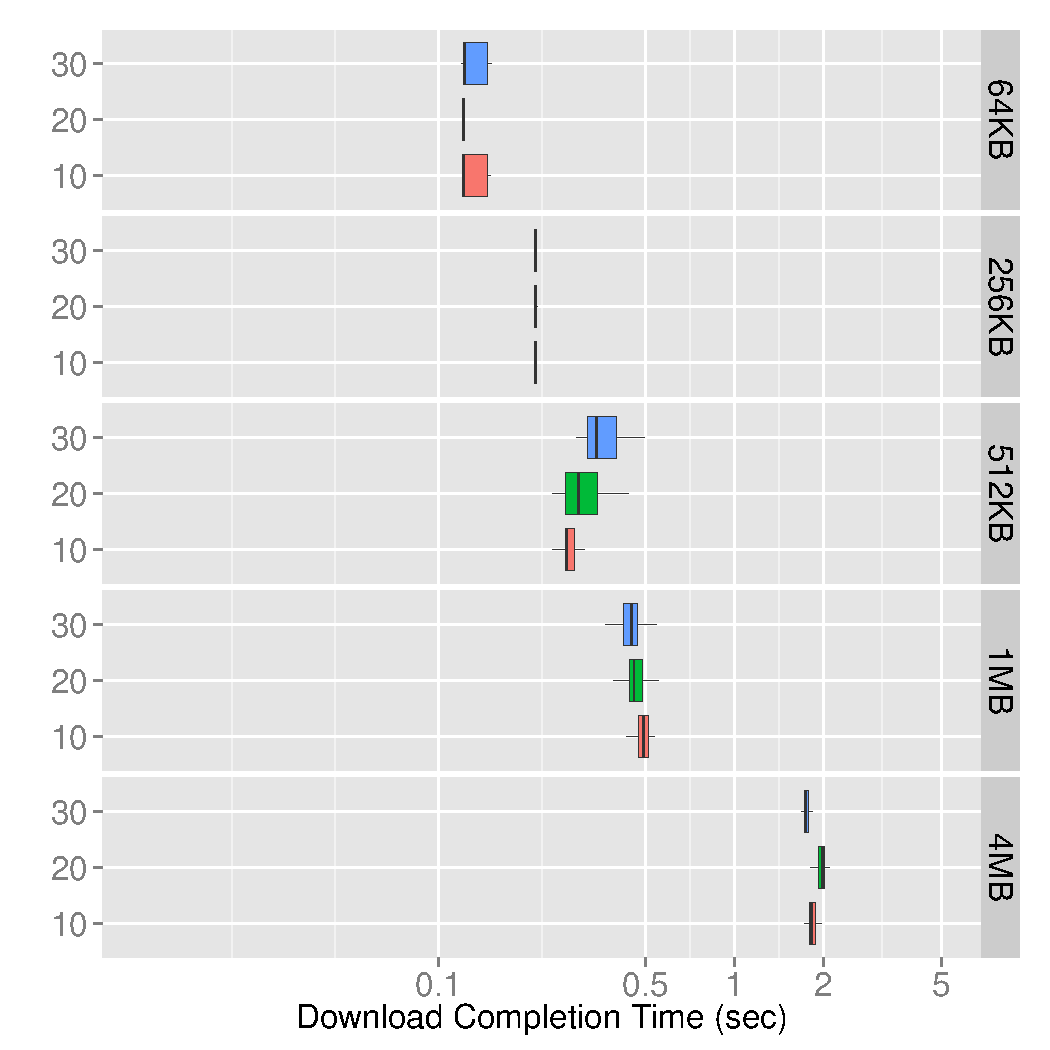
\includegraphics[width=\linewidth]{Figures/dynamic-alpha-alpha.pdf}
		\caption{\label{fig:evaluation-alpha-value-a}Effect of $\alpha_{init}$ in \algalpha~scheduler.}
    \end{center}
    \end{minipage}
\vspace*{-0.3cm}
\end{figure*}

We depict the impact of $\alpha_{init}$ for the \algalpha~scheduler in~\fref{fig:evaluation-alpha-value-a} and the impact of $\alpha_{i,j}$ for the \algslice~scheduler in~\fref{fig:evaluation-alpha-value-b}. 

$\alpha_{init}$ and $\alpha_{i,j}$ are explained in~\xref{sec:alpha-approach} and~\xref{sec:synchronization-approach} respectively. 
In short, a high $\alpha_{init}$ means a high chunk size in the beginning of \algalpha~scheduling and a high $\alpha_{i,j}$ means a high average chunk size during the whole \algslice~scheduling. 

We see that even with changed $\alpha$-values, the performance of the schedulers does not change much. 
On the first view this might be surprising, but can be explained when looking at it closer. 

In case of \algalpha~scheduling, $\alpha_{init}$ merely influences the size of the first chunks. 
Later the chunk size step by step adjusts according to the measured link quality. 
This might be a reason why we do not see a big performance difference between different $\alpha_{init}$ values. 


\begin{figure*}[!htb]
    \begin{minipage}[t]{0.8\linewidth}
    \begin{center}
        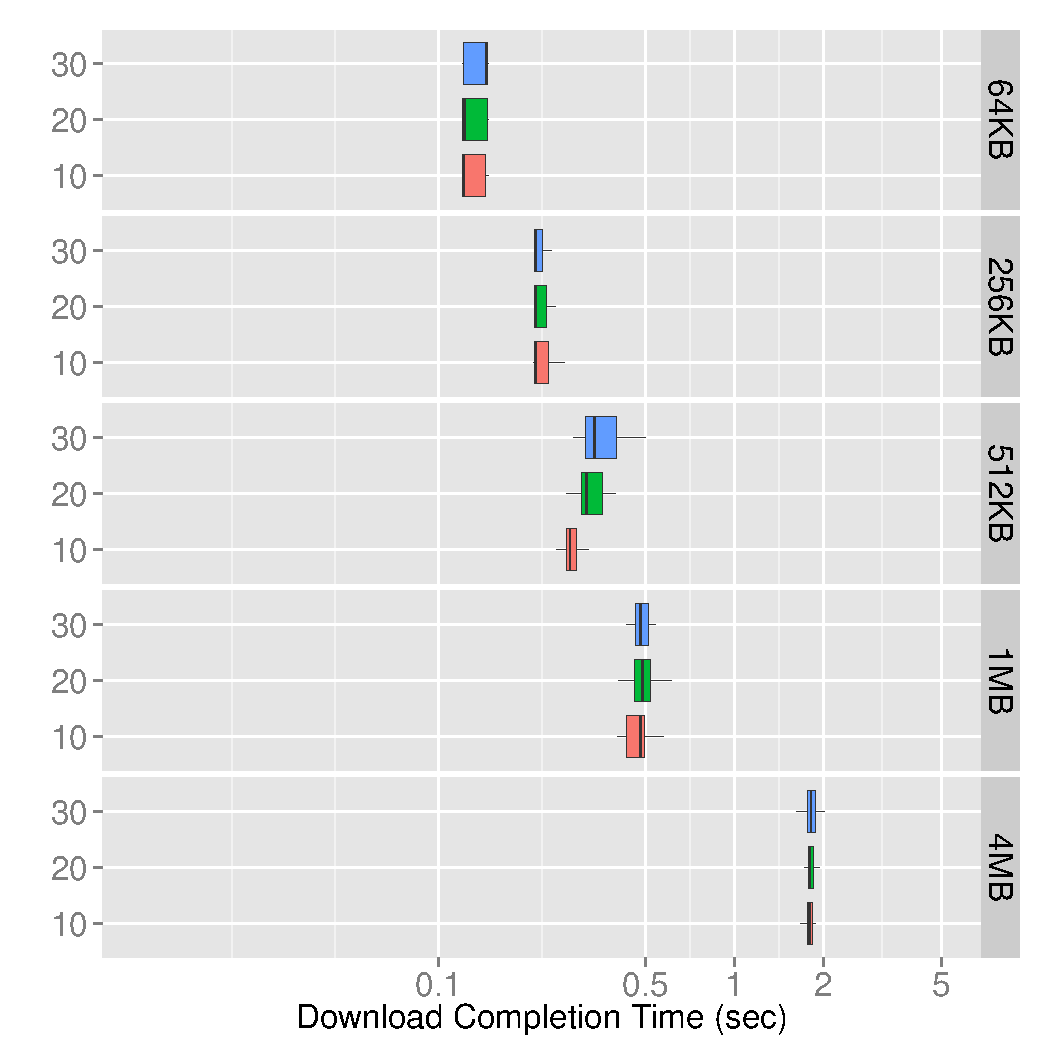
\includegraphics[width=\linewidth]{Figures/dynamic-slice-alpha.pdf}
		\caption{\label{fig:evaluation-alpha-value-b}Effect of $\alpha_{i,j}$ in \algslice~scheduler.}
    \end{center}
    \end{minipage}
  \vspace*{-0.3cm}
\end{figure*}

For \algslice~scheduling, a bigger $\alpha_{i,j}$, means larger chunks in the middle of the download, which consequently also means less overall request overhead. 
In our testbed, bigger $\alpha_{i,j}$ do not make a big difference though. 

To summarize, a high $\alpha_{init}$ might reduce the request overhead in the beginning, but it comes with the risk that we lose adaptiveness to link quality changes. 
This is why from now on we use the intermediate value $\alpha_{init} = 20$ for our further measurements. 
Similarly for $\alpha_{i,j}$, where a high value might reduce request overhead for the loss of link adaptiveness, we also decide to use from now on the intermediate value $\alpha_{i,j} = 20$. 

\pagebreak
\subsection{Comparison of different Schedulers} 
\label{sec:evaluation-schedulers-mixed}

\begin{figure*}[!htb]
    \begin{minipage}[t]{0.8\linewidth}
	\begin{center}
        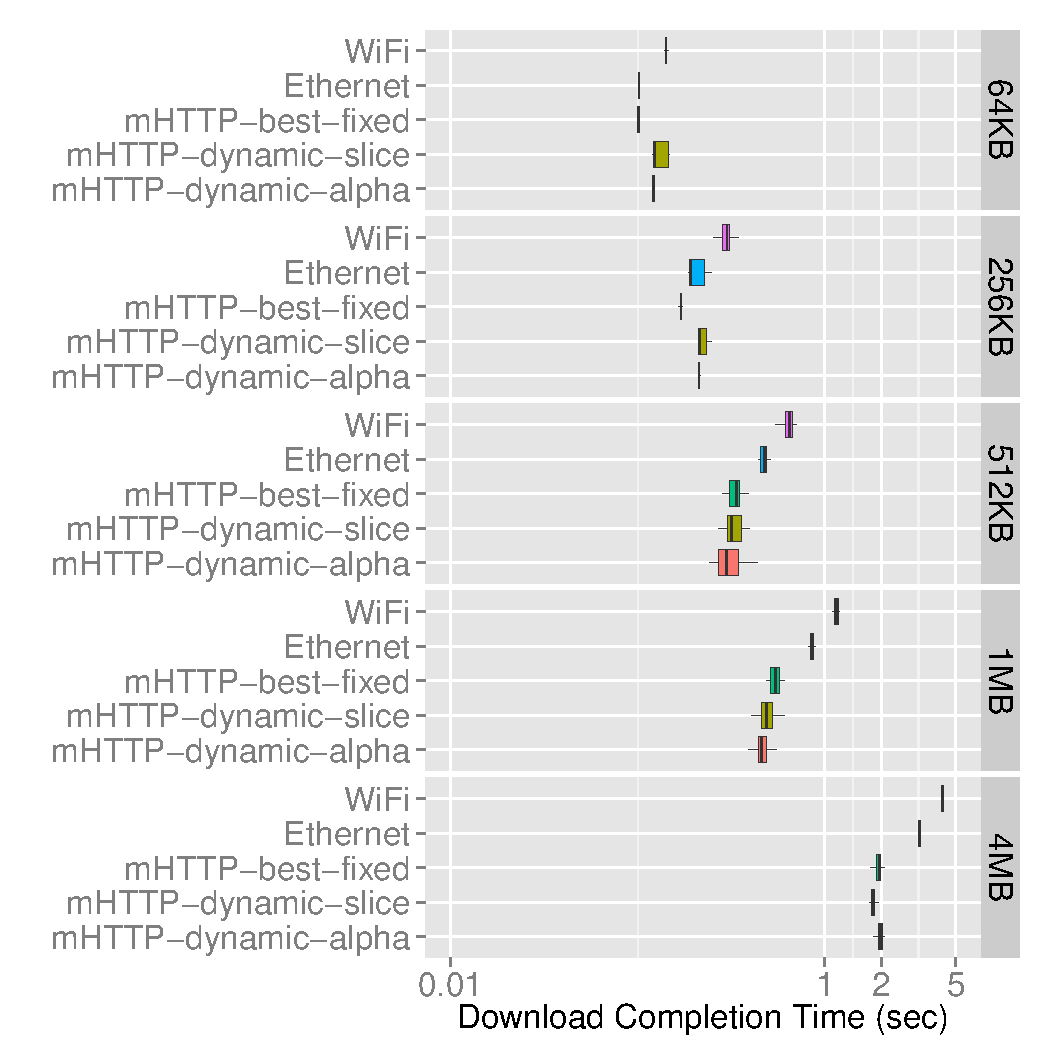
\includegraphics[width=\linewidth]{Figures/scheduler-comparison.pdf}
		\caption{\label{fig:evaluation-comparison-times}Download times of different scheduler algorithms.}
    \end{center}
    \end{minipage}
\vspace*{-0.3cm}
\end{figure*}

In~\fref{fig:evaluation-comparison-times} we depict the download times of different files for each scheduler, \ie \algalpha~(dynamic-alpha), \algslice~(dynamic-slice) and the \algbase~scheduler (best-fixed). 
Also, we show the download times of each single interface, \ie \ethernet~and \wifi.
$\alpha_{init}$ and $\alpha_{i,j}$ are both set to $20$, as previously explained in~\xref{sec:evaluation-alpha}. 
Further, as discussed in~\xref{sec:evaluation-initial-chunk}, the initial chunk size is set to $32$KB.
Please note that the depicted results of the \algbase~scheduler are the best performing fixed chunk sizes for our testbed, meaning all other fixed chunk sizes performed worse than these results. 
We can see that on small files, such as $64-256$KB, our developed schedulers perform nearly as good as the best fixed chunk size. 
The slight difference between them can be explained through the extra request overhead, since our new schedulers tend to perform more requests on small files due to the small initial chunk size. 
Starting from $512$KB our new schedulers even tend to perform slightly better than the best fixed chunk size. 


\begin{figure*}[!htb]
    \begin{minipage}[t]{0.8\linewidth}
    \begin{center}
        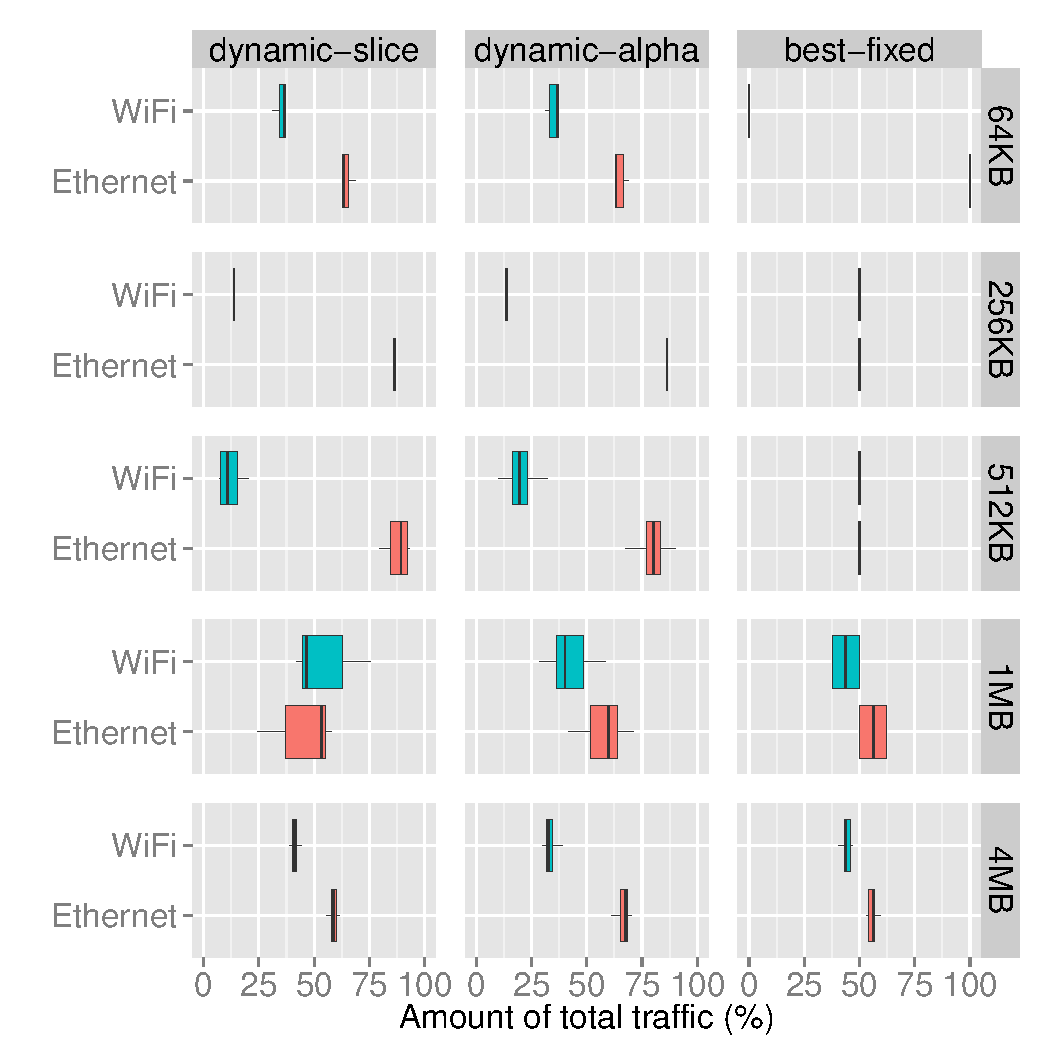
\includegraphics[width=\linewidth]{Figures/traffic-distribution-all.pdf}
		\caption{\label{fig:evaluation-comparison-traffic}Traffic distributions among the paths.}
    \end{center}
    \end{minipage}
  \vspace*{-0.3cm}
\end{figure*}

When looking at the traffic distribution among the paths, as depicted in~\fref{fig:evaluation-comparison-traffic}, we see that the fixed chunk size scheduler tends to distribute the traffic equally, whereas our new developed schedulers distribute the traffic according to the links' qualities. 
Especially in case of $256$KB and $512$KB file downloads, we can see that the fixed chunk scheduler does not take link qualities into account and distributes the chunks evenly over the paths. 
In case of the $64$KB file download, the fixed chunk size is big enough to download the whole file in one chunk, resulting in the whole traffic being processed over the \ethernet~link, while the \wifi~link stays idle. 
In the traffic distribution for $1$MB file downloads with the \algslice~scheduler, we see that in a few scenarios more traffic has been scheduled over the supposedly weaker interface, \ie~the \wifi~interface. 
It is hard to find the exact reason for this behavior, but since the download time in this case is similar to the one with the \algalpha~scheduler, we see that the scheduler made the correct choices at that time. 

Overall the \algalpha~and the \algslice~scheduler perform very similar, in both traffic distribution and download time. 
One reason for this might be, that the \algslice~scheduler tends to have smaller chunks towards the end of the download. 
The gain attained from the synchronization might get neglected due to this extra request overhead. 

Even though in this experiment both advanced schedulers behave similar, we expect the \algslice~scheduler to be superior in very unstable mobile environments. 
Note, that the links in our German testbed have a relatively stable performance. 
We expect the \algslice~scheduler to behave better in very unstable environments, since it takes an extra constraint into account, \ie the assumption that both connections should finish downloading their last chunk at the same time.
In~\chref{ch:discussion} we talk about future mobility studies, in which we expect the \algslice~algorithm to perform better than the \algalpha~scheduler. 
In the following evaluations we use the \algslice~scheduler as \mhttp's default scheduler. 

\subsection{mHTTP vs. MPTCP}
\label{sec:evaluation-mptcp}

\begin{figure*}[!htb]
    \begin{minipage}[t]{0.8\linewidth}
	\begin{center}
        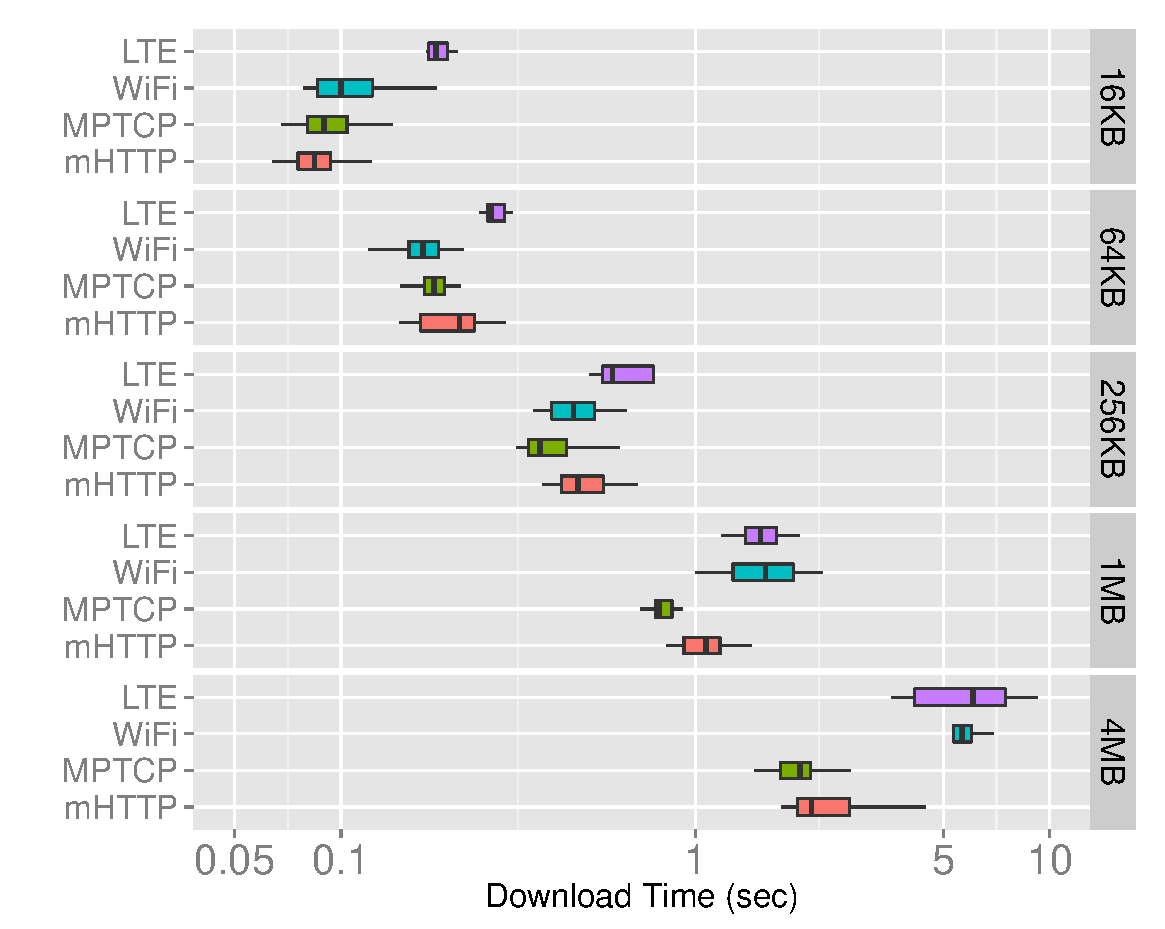
\includegraphics[width=\linewidth]{Figures/umass-mhttp-mptcp-stcp-32k.pdf}
		\caption{\label{fig:evaluation-mptcp-times}Download times of \mhttp~vs. MPTCP vs. HTTP.}
    \end{center}
    \end{minipage}
\vspace*{-0.3cm}
\end{figure*}

We use the \algslice~scheduler to compare \mhttp~with MPTCP, due to the reasons explained in~\xref{sec:evaluation-schedulers-mixed}.
$\alpha_{init}$ and $\alpha_{i,j}$ are both set to $20$, as previously explained in~\xref{sec:evaluation-alpha}. 
Further, as discussed in~\xref{sec:evaluation-initial-chunk}, the initial chunk size is set to $32$KB.
For the experiment we use our US testbed as explained in~\xref{sec:evaluation-testbed}. 

\begin{figure*}[!htb]
    \begin{minipage}[t]{0.8\linewidth}
    \begin{center}
        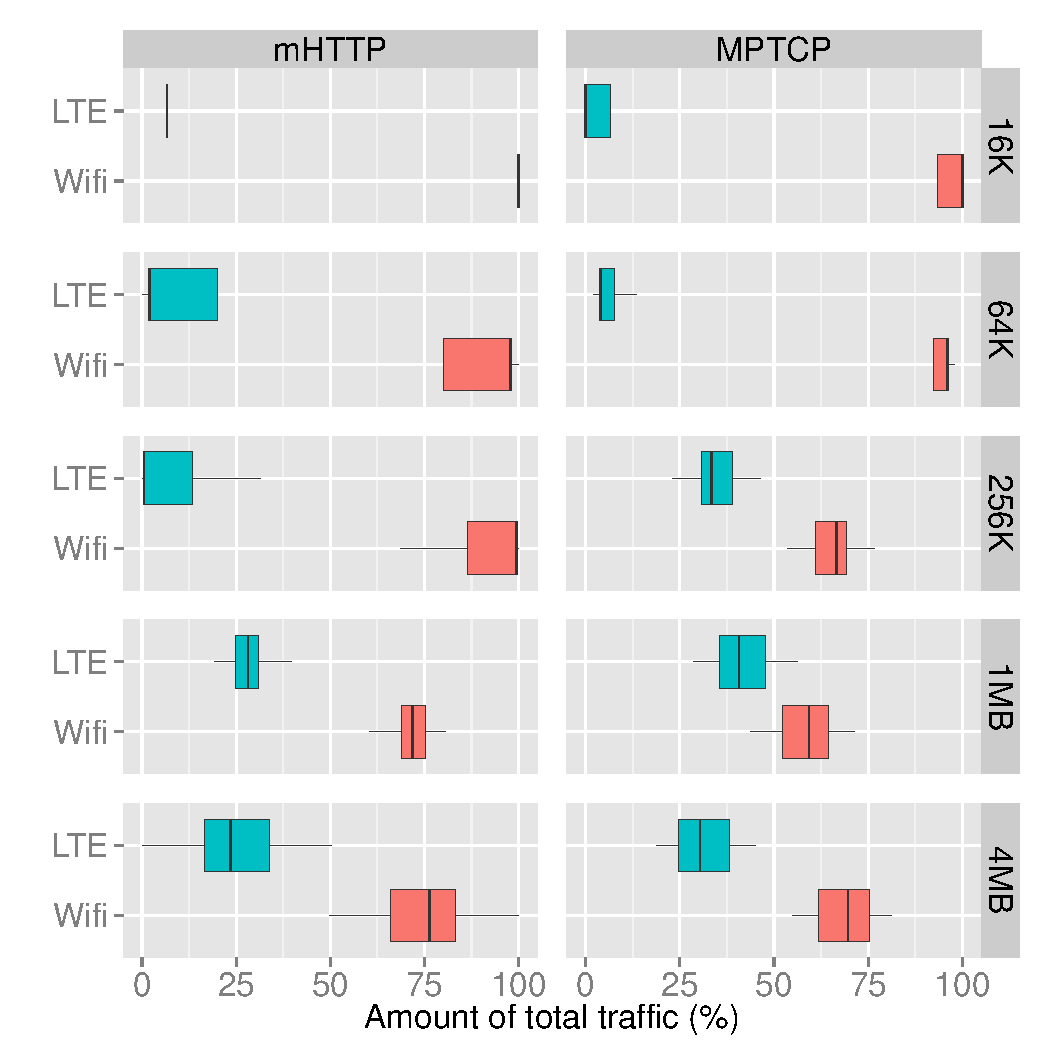
\includegraphics[width=\linewidth]{Figures/umass-mhttp-mptcp-stcp-fraction.pdf}
		\caption{\label{fig:evaluation-mptcp-traffic}Traffic distribution of \mhttp~vs. MPTCP.}
    \end{center}
    \end{minipage}
  \vspace*{-0.3cm}
\end{figure*}

The results of the download times are shown in~\fref{fig:evaluation-mptcp-times}. 
We see that MPTCP performs slightly better than \mhttp~with \algslice~scheduling. 
However, the difference between both is small, especially in the $4$MB download case. 
It is important to mention, that our US testbed is optimized for MPTCP beyond the default MPTCP standard. 
The proposed standard uses coupled congestion control~\cite{RFC-6356}, whereas our testbed uses uncoupled congestion control with Cubic~\cite{TCP-CUBIC}, meaning that in the standard case MPTCP would likely perform worse than what we observe here \cite{CHEN13-MSM}. 

In~\fref{fig:evaluation-mptcp-traffic}, we illustrate the traffic distribution of \mhttp~and MPTCP over the available network interfaces. 
We see that MPTCP transmits a larger fraction of traffic over the \lte~interface, especially in case of small files (\eg $256$KB). 
This might explain, why MPTCP performs slightly better here. 
For $4$MB files, the difference in traffic distribution is negligible. 

\pagebreak
